\begin{figure}[t]
\centering
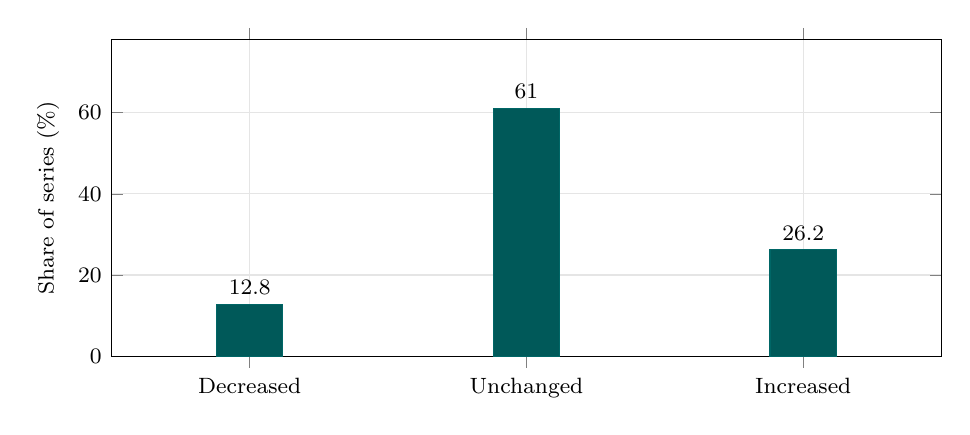
\begin{tikzpicture}
\begin{axis}[
  ybar,
  width=\columnwidth,
  height=5.6cm,
  ymin=0, ymax=78,
  ylabel={Share of series (\%)},
  symbolic x coords={Decreased,Unchanged,Increased},
  xtick=data,
  nodes near coords,
  every node near coord/.append style={font=\footnotesize},
  bar width=24pt,
  enlarge x limits=0.25,
  tick label style={font=\footnotesize},
  label style={font=\footnotesize},
  grid=major,
  major grid style={gray!20},
]
\addplot[fill=teal!70!black, draw=teal!80!black] coordinates {
  (Decreased,12.8)
  (Unchanged,61.0)
  (Increased,26.2)
};
\end{axis}
\end{tikzpicture}
\caption{Change in dependency and layering violations over 12 months after the introduction of parseable ArchUnit constraints.}
\label{fig:rq4_change}
\end{figure}
